\begin{frame}[label=p4_20260916]{Configuration 1: selected mass spectrum and fit}
  \relax
  {\small Relative weighted X-MC efficiency: 25\%; score $>0.95279$.}\par
  \begin{columns}[T]
    \column{0.48\textwidth}\centering
    {\small\textbf{cut\_scan: selected DATA}}\par
    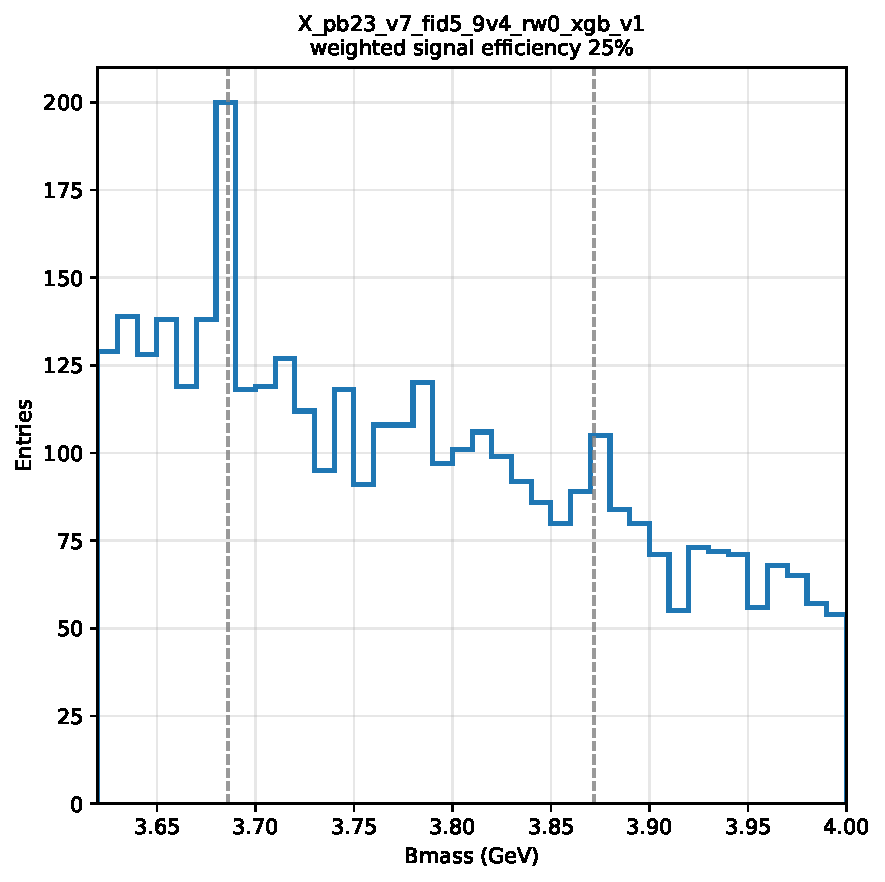
\includegraphics[width=\linewidth,height=0.52\textheight,keepaspectratio]{figures/20260916/config1_cut_scan.pdf}
    \column{0.48\textwidth}\centering
    {\small\textbf{Default single-X fit}}\par
    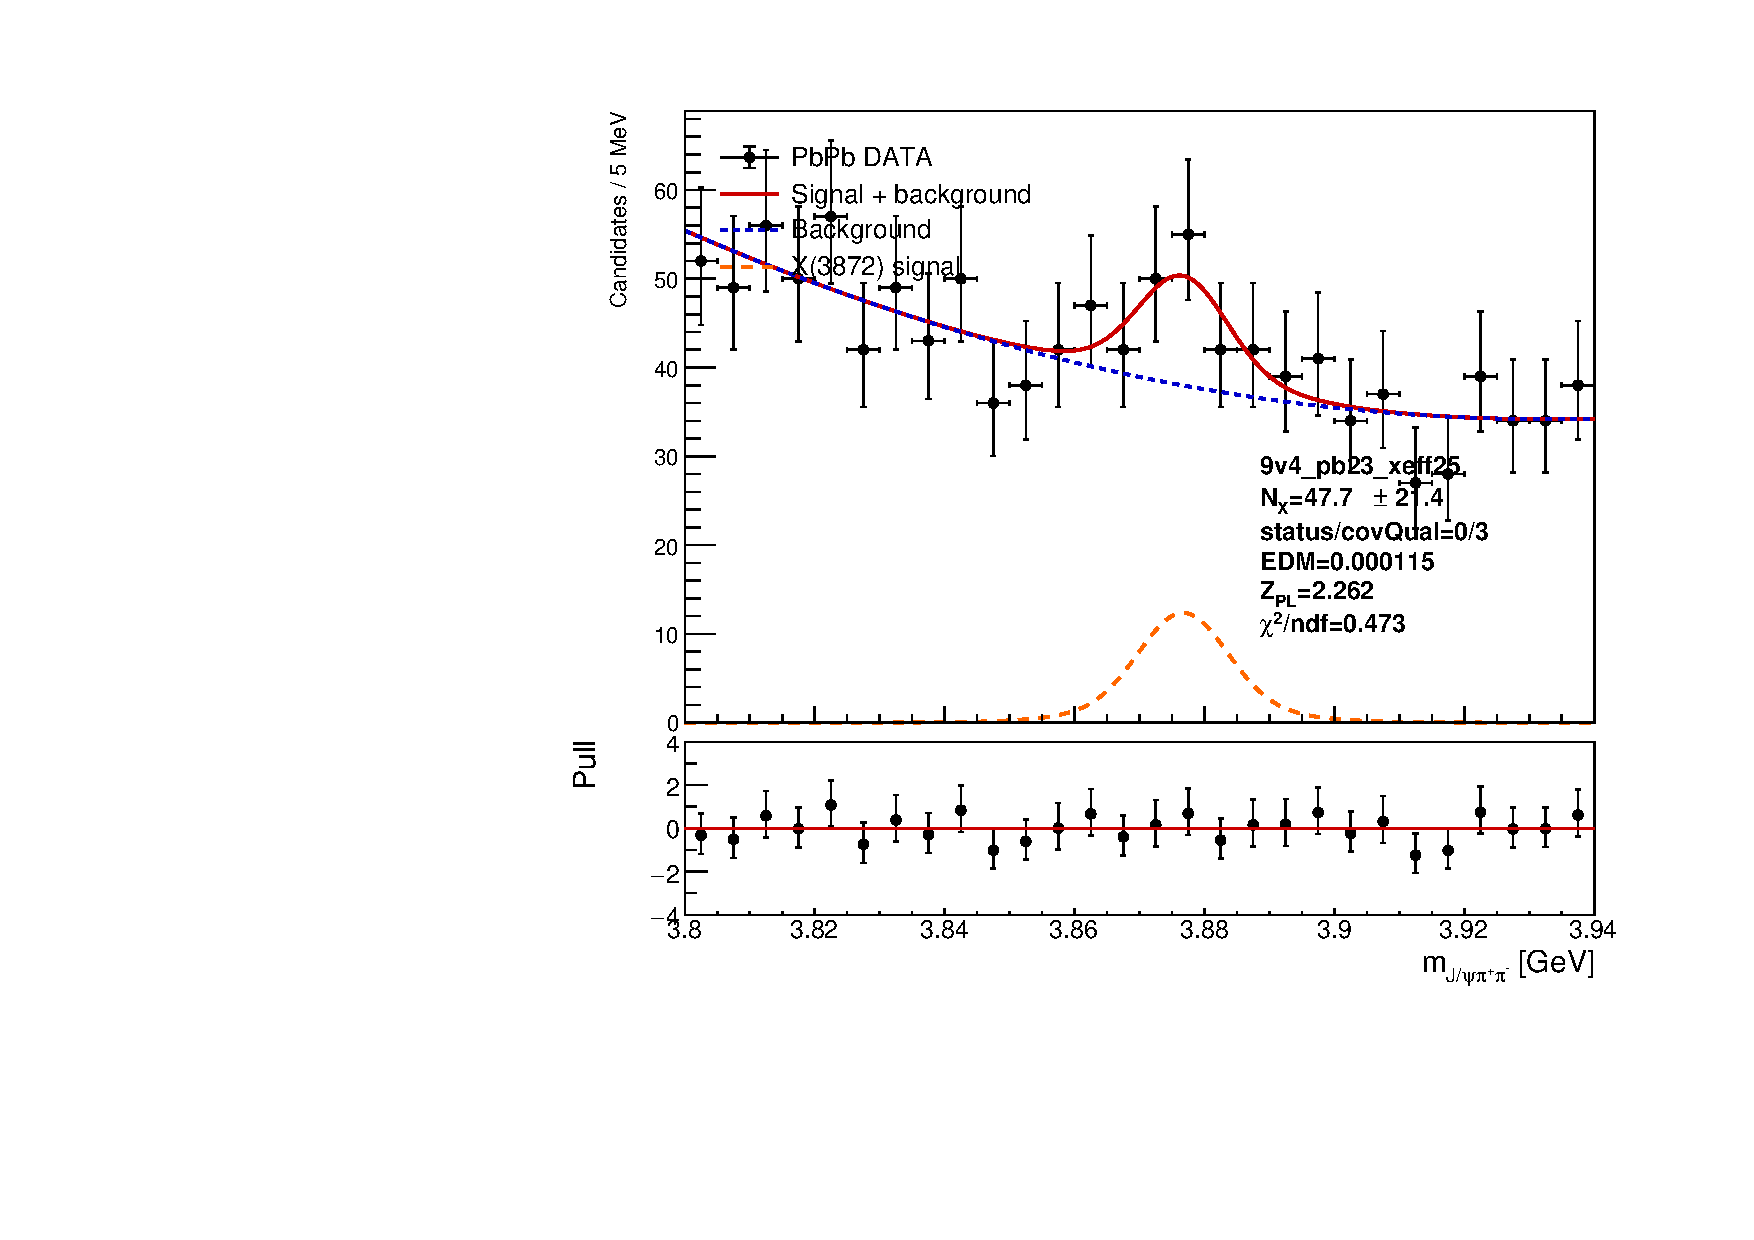
\includegraphics[width=\linewidth,height=0.52\textheight,keepaspectratio]{figures/20260916/config1_fit.pdf}
  \end{columns}
  {\small $N_X=47.71\pm21.44$;\quad $\mu_X=3876.69\pm7.51$ MeV;\quad scale $=1.500$.}\par
  {\small Significance: $2.262$.}\par
  \caution{Mean and scale at their upper bounds. Fit range: 3.80--3.94 GeV.}
\end{frame}

\begin{frame}[label=p5_20260916]{Configuration 2: selected mass spectrum and fit}
  \relax
  {\small Relative weighted X-MC efficiency: 40\%; score $>0.86855$.}\par
  \begin{columns}[T]
    \column{0.48\textwidth}\centering
    {\small\textbf{cut\_scan: selected DATA}}\par
    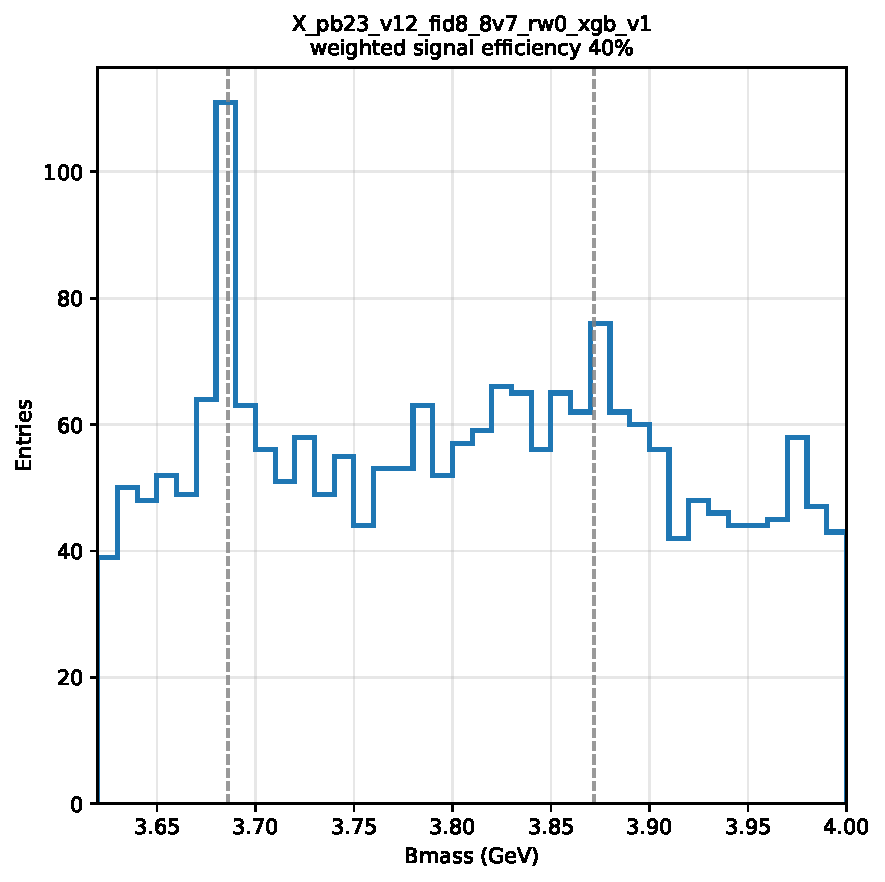
\includegraphics[width=\linewidth,height=0.52\textheight,keepaspectratio]{figures/20260916/config2_cut_scan.pdf}
    \column{0.48\textwidth}\centering
    {\small\textbf{Default single-X fit}}\par
    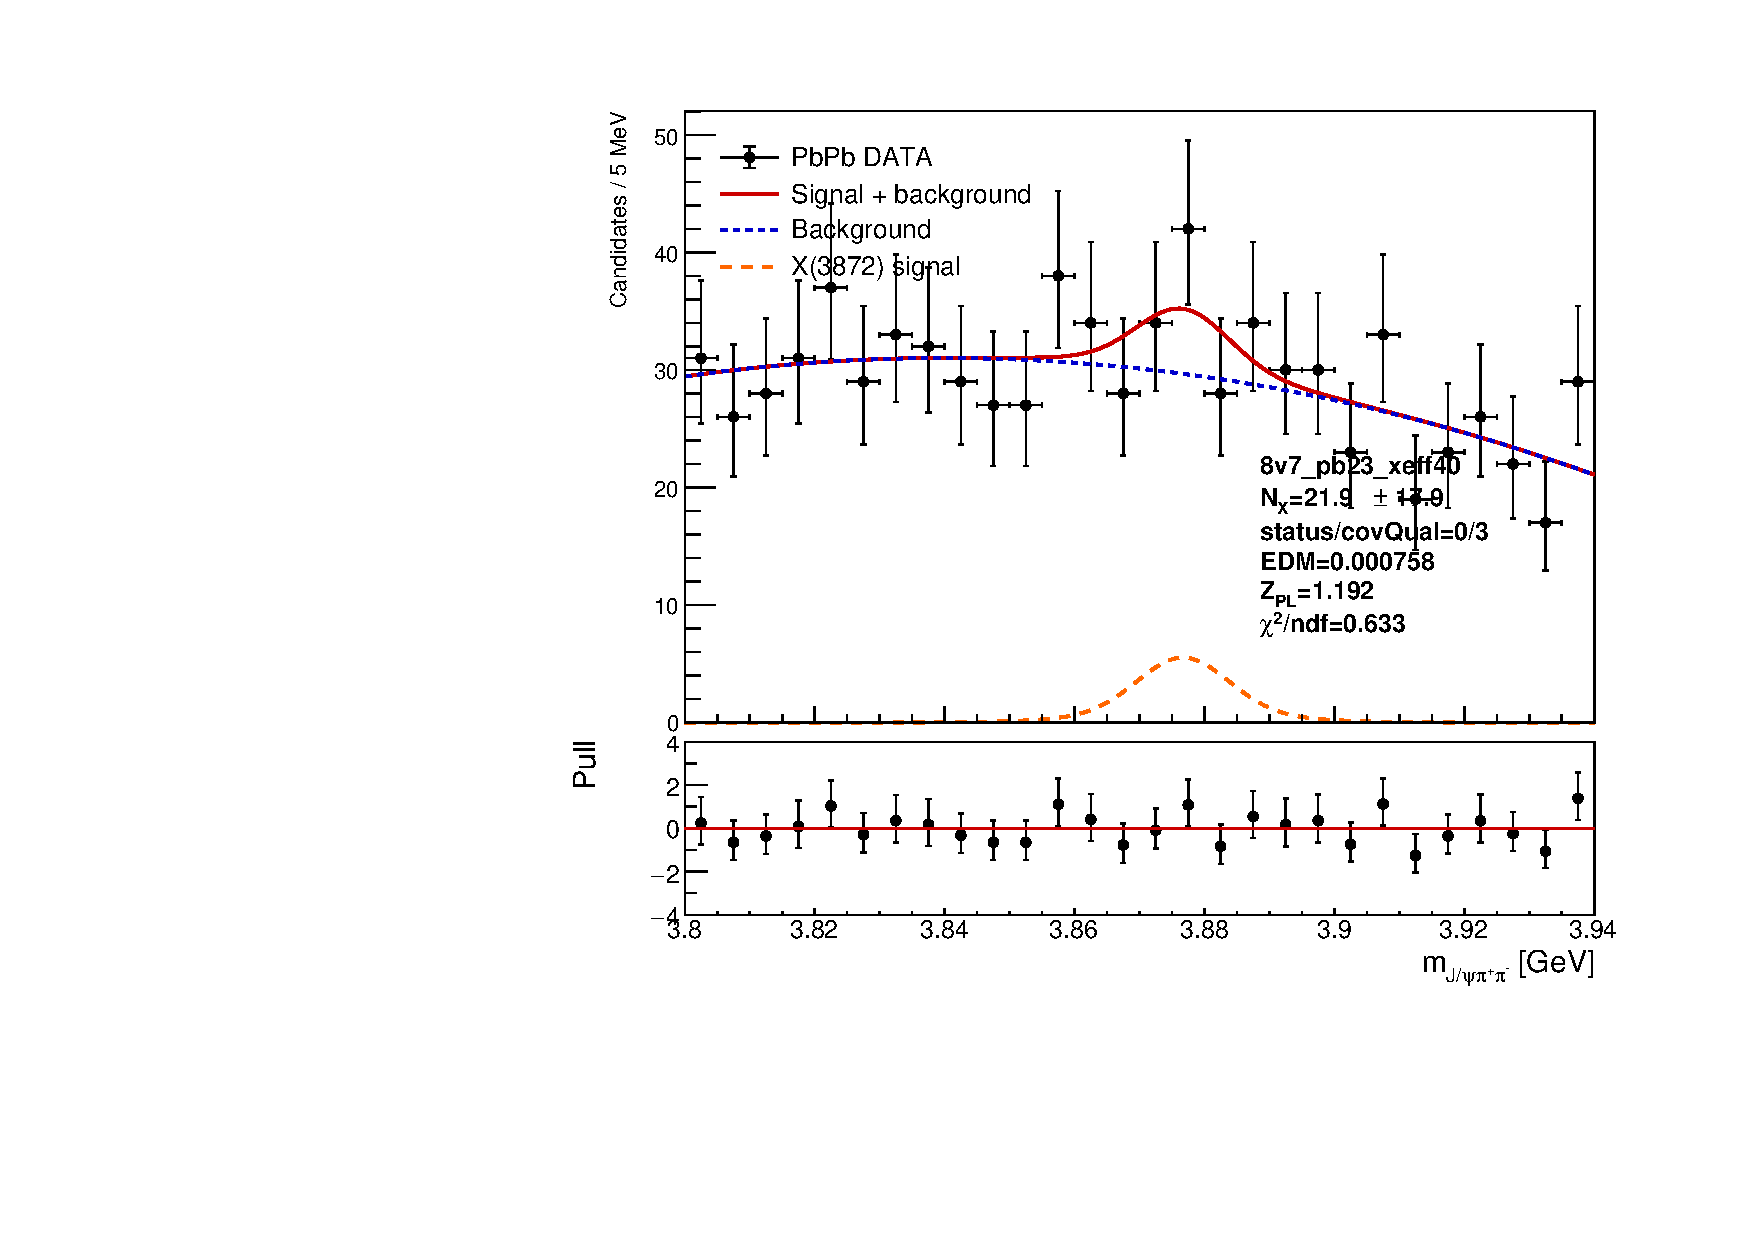
\includegraphics[width=\linewidth,height=0.52\textheight,keepaspectratio]{figures/20260916/config2_fit.pdf}
  \end{columns}
  {\small $N_X=21.94\pm17.92$;\quad $\mu_X=3876.69\pm6.90$ MeV;\quad scale $=1.500$.}\par
  {\small Significance: $1.192$.}\par
  \caution{Mean and scale at their upper bounds. Fit range: 3.80--3.94 GeV.}
\end{frame}

\begin{frame}[label=p6_20260916]{Configuration 3: selected mass spectrum and fit}
  \relax
  {\small Relative weighted X-MC efficiency: 25\%; score $>0.95267$.}\par
  \begin{columns}[T]
    \column{0.48\textwidth}\centering
    {\small\textbf{cut\_scan: selected DATA}}\par
    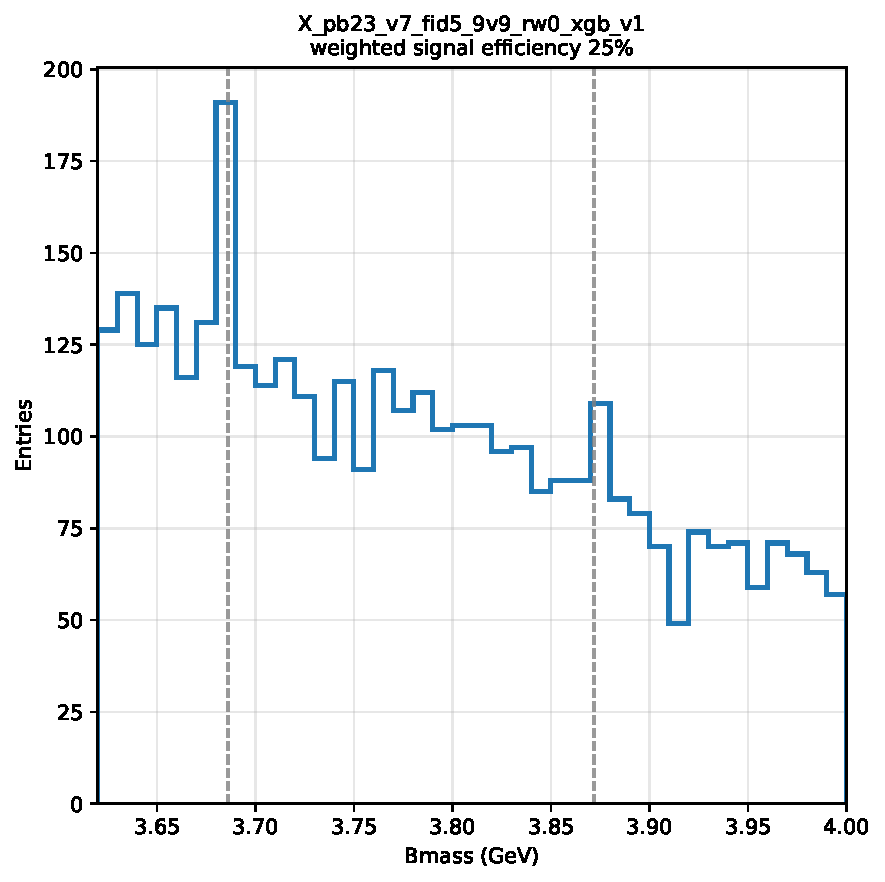
\includegraphics[width=\linewidth,height=0.52\textheight,keepaspectratio]{figures/20260916/config3_cut_scan.pdf}
    \column{0.48\textwidth}\centering
    {\small\textbf{Default single-X fit}}\par
    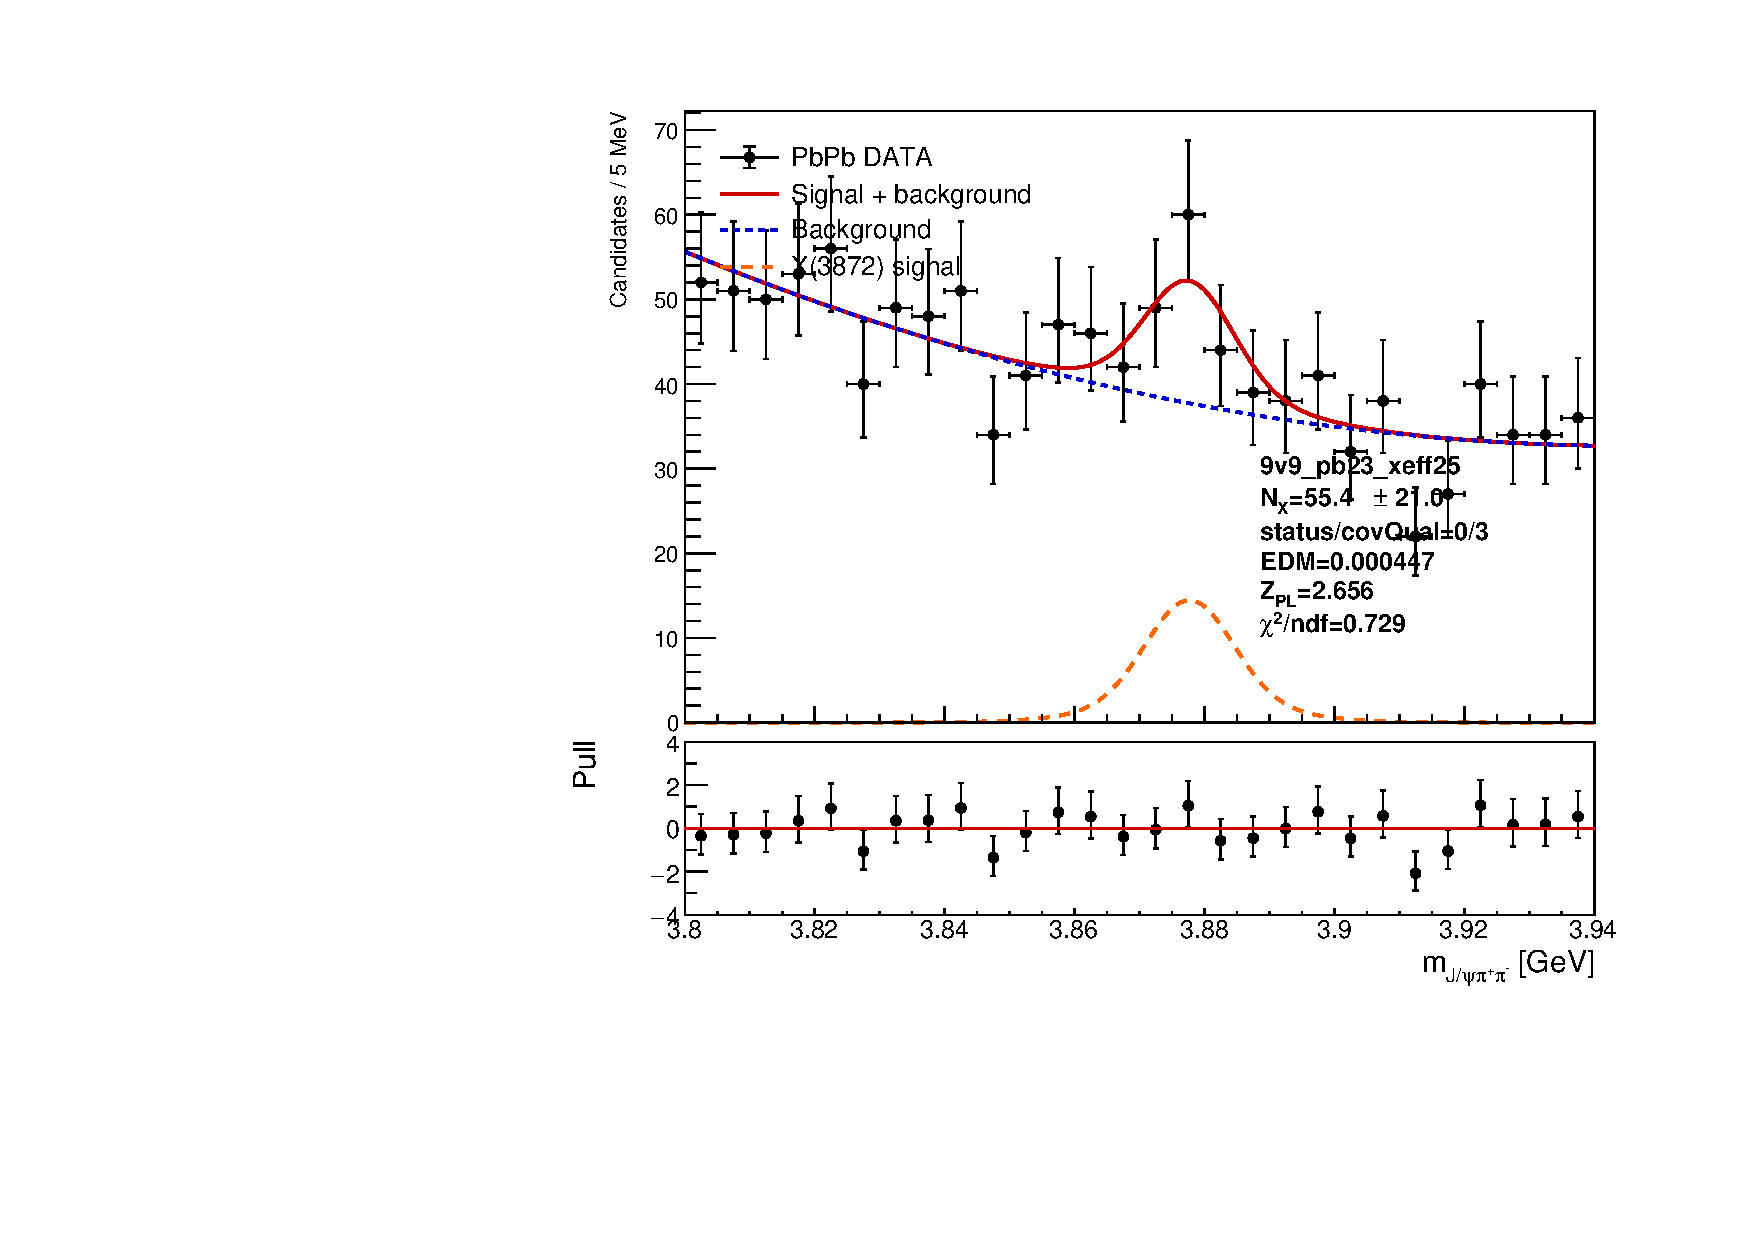
\includegraphics[width=\linewidth,height=0.52\textheight,keepaspectratio]{figures/20260916/config3_fit.pdf}
  \end{columns}
  {\small $N_X=55.42\pm21.04$;\quad $\mu_X=3877.67\pm2.82$ MeV;\quad scale $=1.495$.}\par
  {\small Significance: $2.656$.}\par
  \caution{Mean range: nominal $\pm10$ MeV; scale range: [0.5,1.5]. Fit range: 3.80--3.94 GeV.}
\end{frame}

\begin{frame}[label=p7_20260916]{Configuration 4: selected mass spectrum and fit}
  \relax
  {\small Relative weighted X-MC efficiency: 40\%; score $>0.84505$.}\par
  \begin{columns}[T]
    \column{0.48\textwidth}\centering
    {\small\textbf{cut\_scan: selected DATA}}\par
    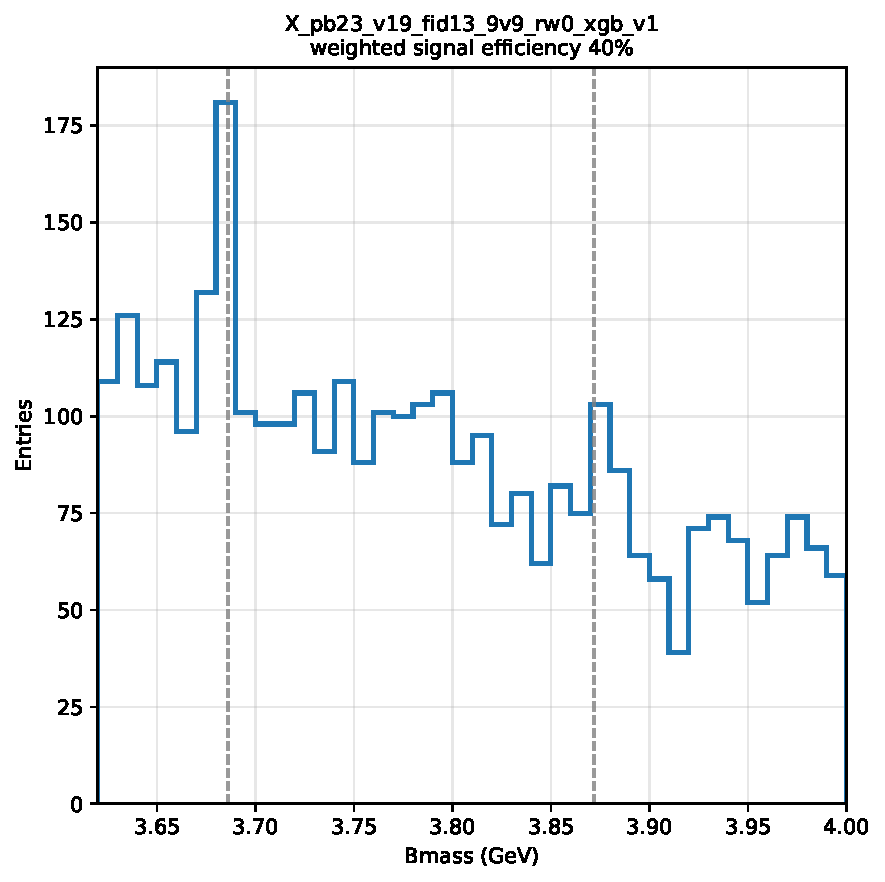
\includegraphics[width=\linewidth,height=0.52\textheight,keepaspectratio]{figures/20260916/config4_cut_scan.pdf}
    \column{0.48\textwidth}\centering
    {\small\textbf{Two-peak fit}}\par
    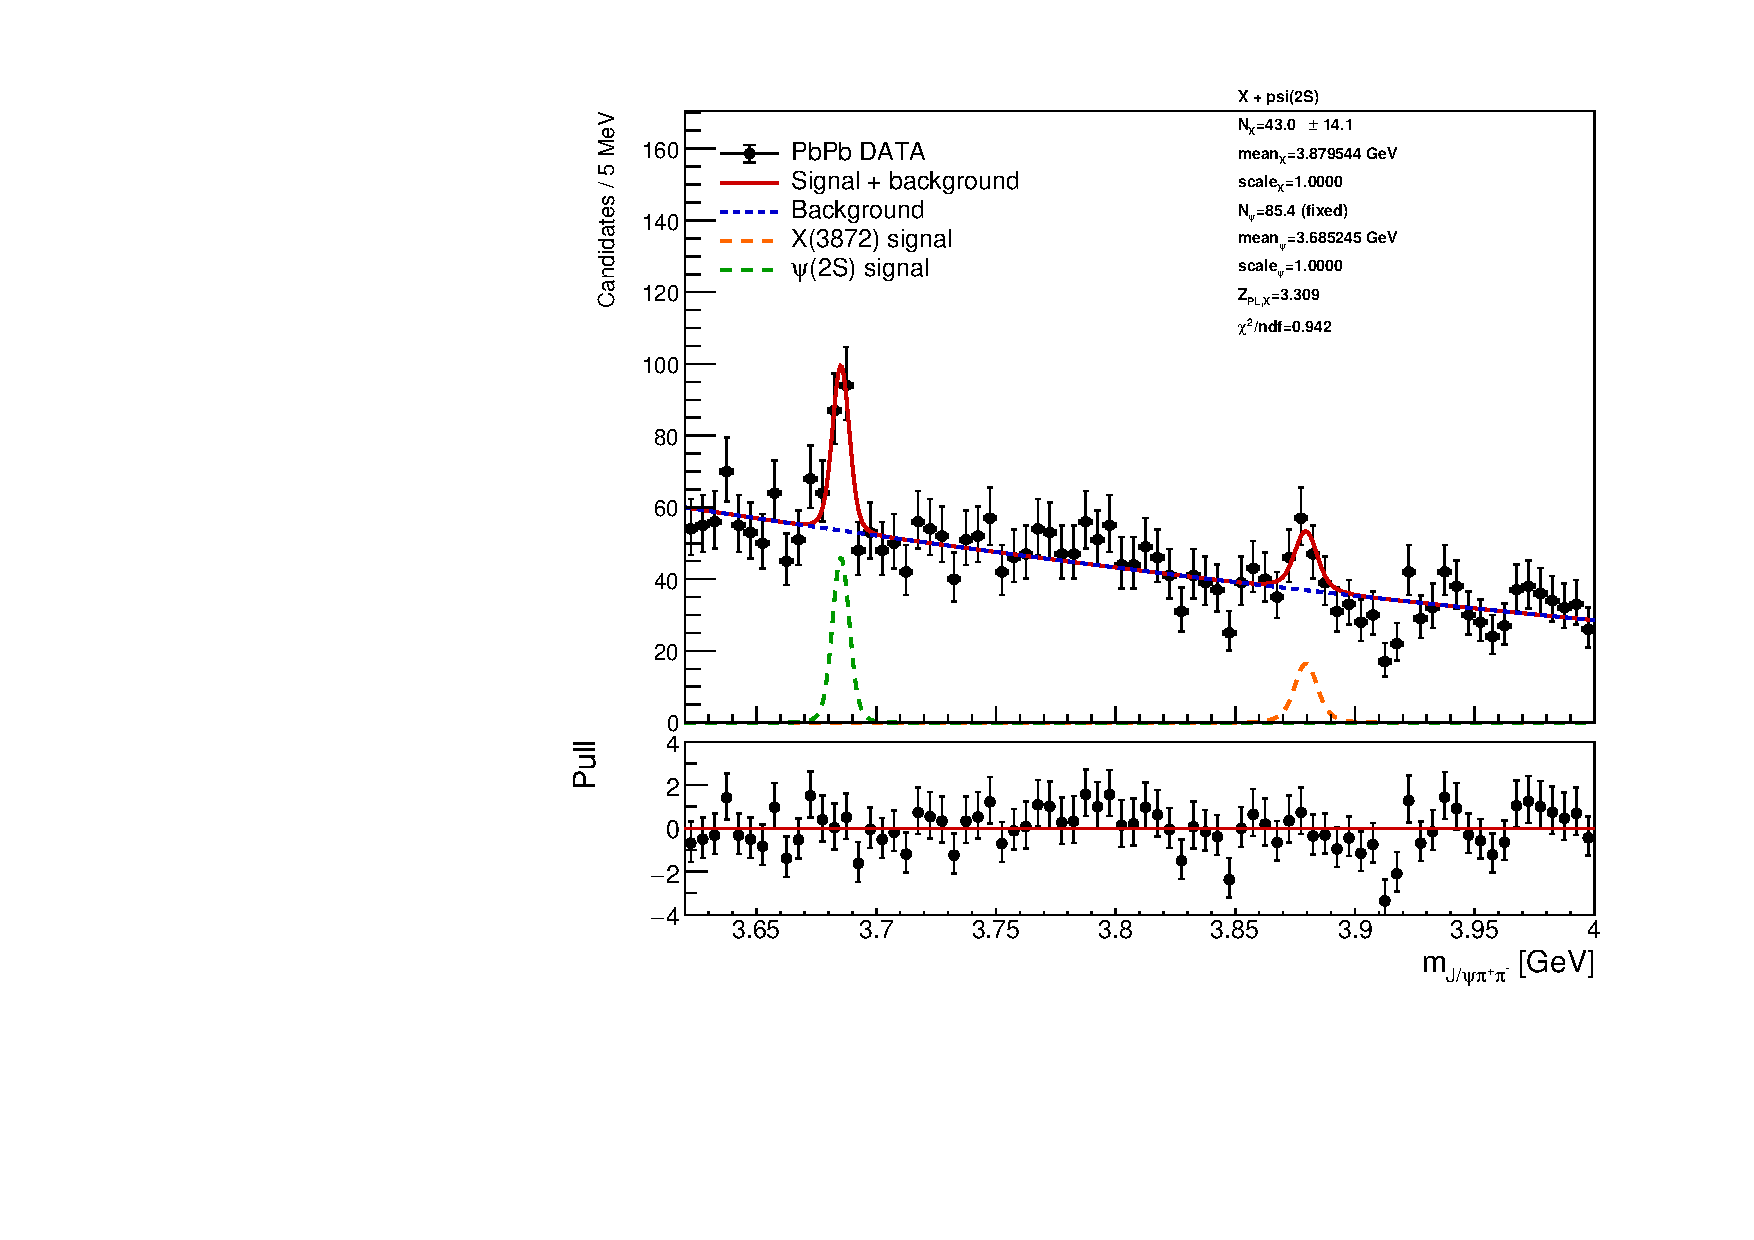
\includegraphics[width=\linewidth,height=0.52\textheight,keepaspectratio]{figures/20260916/config4_fit.pdf}
  \end{columns}
  {\small $N_X=42.98\pm14.11$;\quad $\mu_X=3879.54$ MeV.}\par
  {\small $N_\psi=85.41$;\quad $\mu_\psi=3685.24$ MeV.}\par
  {\small Significance: $3.309$.}\par
  \caution{Means and $N_\psi$ fixed from the first fit; both scales fixed to 1.}
\end{frame}

\begin{frame}[label=p8_20260916]{Configuration 5: selected mass spectrum and fit}
  \relax
  {\small Relative weighted X-MC efficiency: 50\%; score $>0.78272$.}\par
  \begin{columns}[T]
    \column{0.48\textwidth}\centering
    {\small\textbf{cut\_scan: selected DATA}}\par
    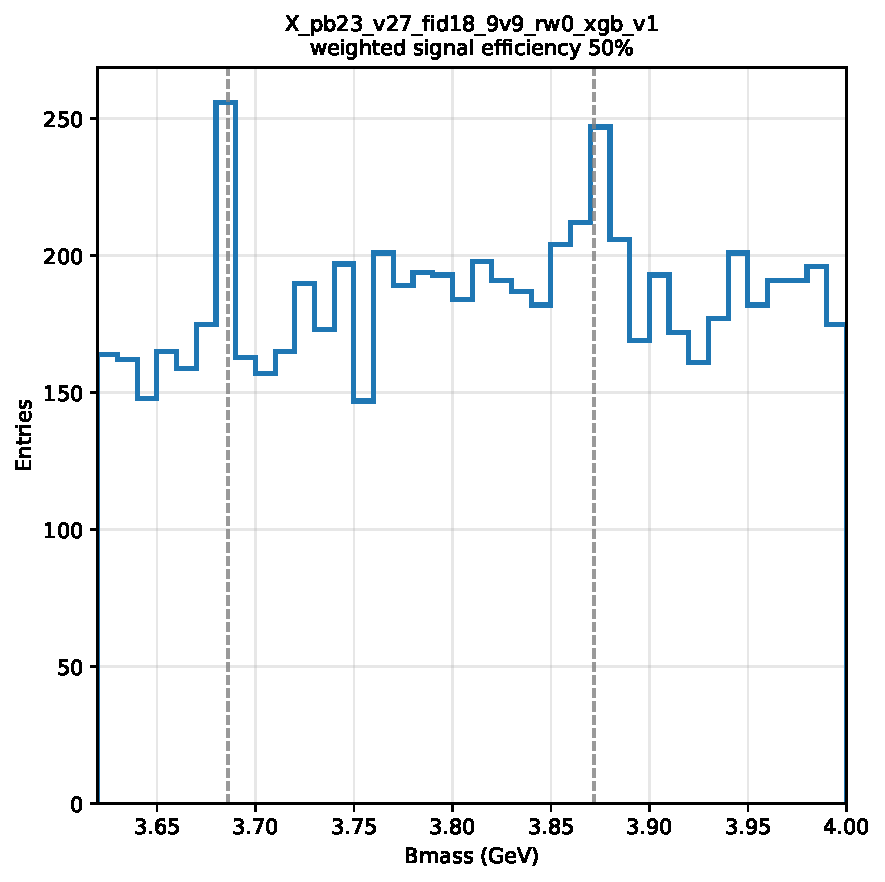
\includegraphics[width=\linewidth,height=0.52\textheight,keepaspectratio]{figures/20260916/config5_cut_scan.pdf}
    \column{0.48\textwidth}\centering
    {\small\textbf{Two-peak fit}}\par
    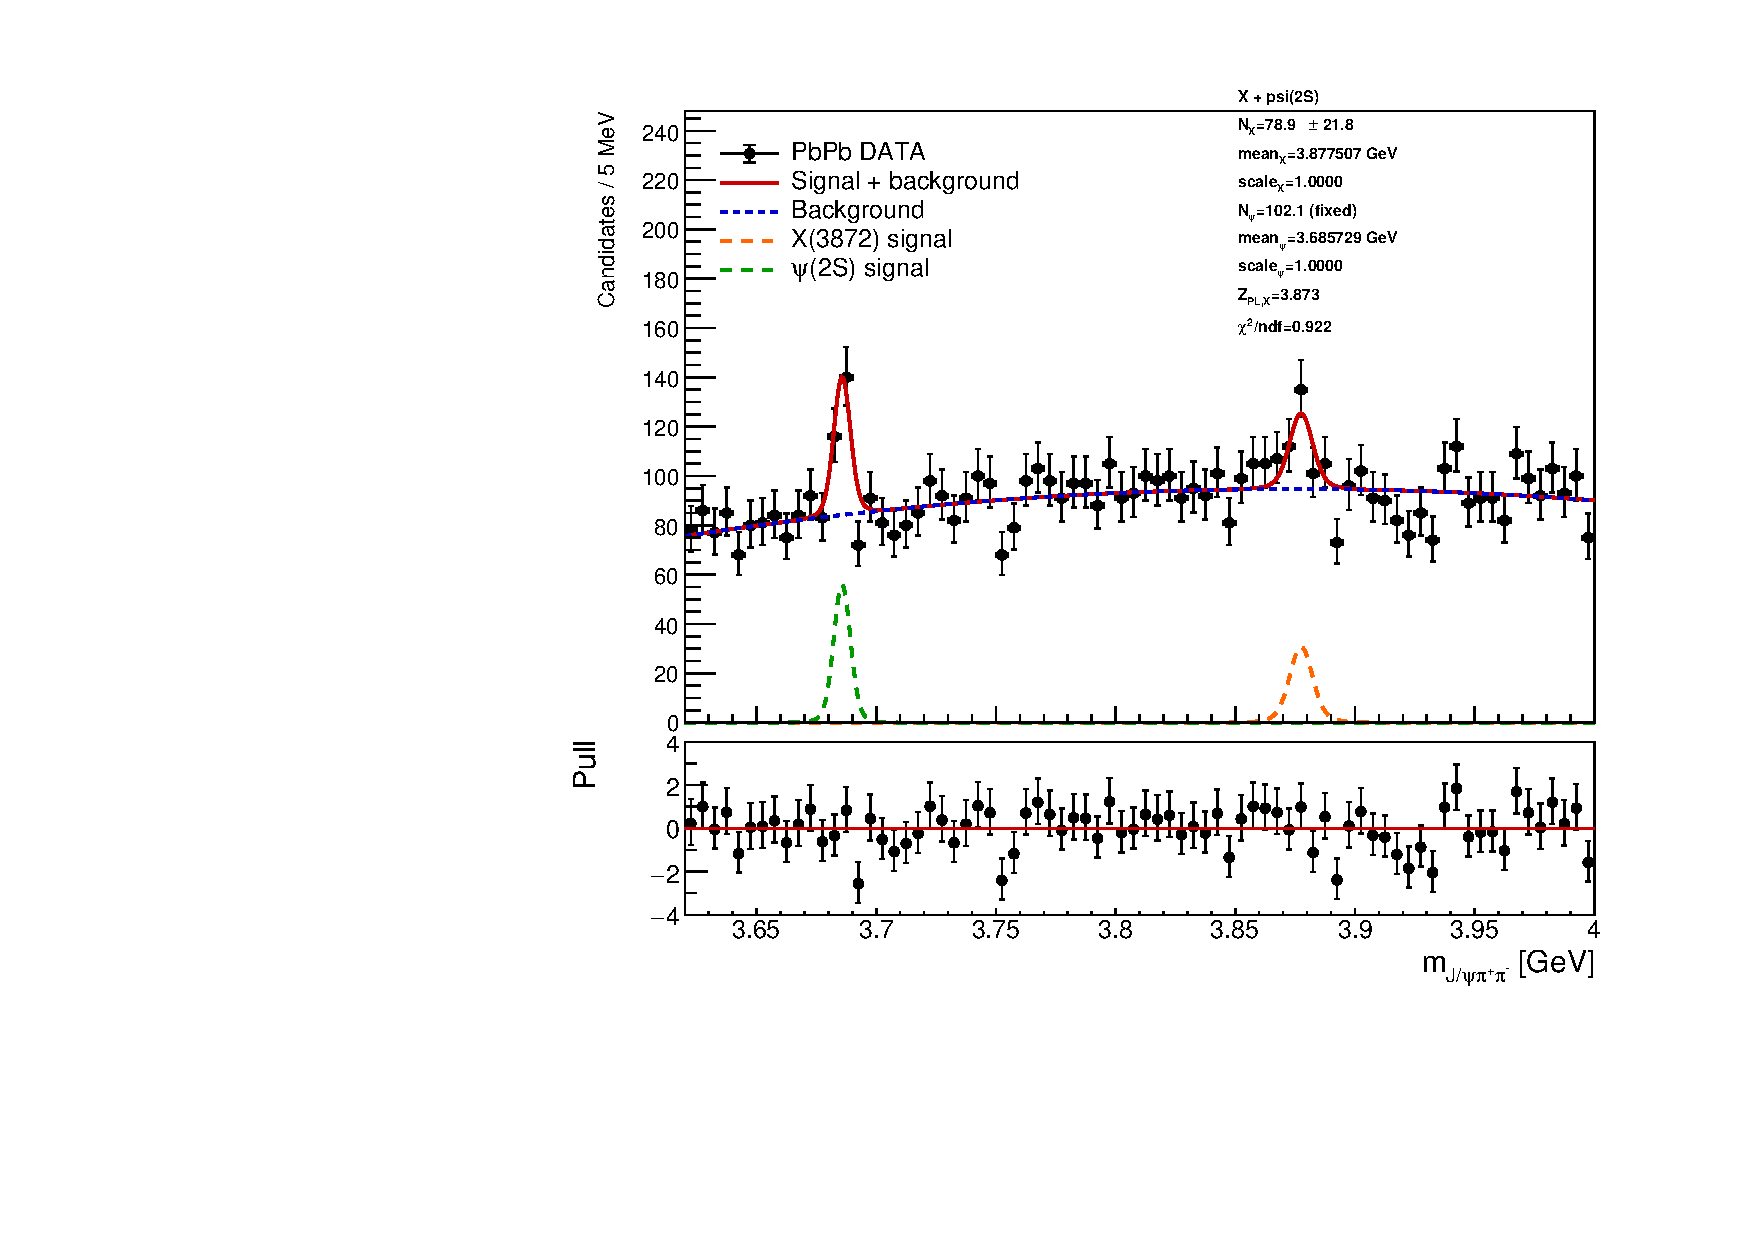
\includegraphics[width=\linewidth,height=0.52\textheight,keepaspectratio]{figures/20260916/config5_fit.pdf}
  \end{columns}
  {\small $N_X=78.88\pm21.76$;\quad $\mu_X=3877.51$ MeV.}\par
  {\small $N_\psi=102.07$;\quad $\mu_\psi=3685.73$ MeV.}\par
  {\small Significance: $3.873$.}\par
  \caution{Means and $N_\psi$ fixed from the first fit; both scales fixed to 1.}
\end{frame}
